% !LW recipe = tectonic
% Main editable submission. Compile from this directory using `make pdf`.
\documentclass[11pt]{article}
\usepackage[paperwidth=13.333in,paperheight=7.5in,left=.56in,right=.56in,top=.74in,bottom=.56in,headheight=14pt,headsep=18pt]{geometry}
\usepackage{fontspec}
\setmainfont{Arial}
\usepackage{xcolor,tabularx,array,booktabs,fancyhdr,pdfpages}
\usepackage[unicode,colorlinks=true,urlcolor=tealink,linkcolor=tealink]{hyperref}
\definecolor{ink}{HTML}{173443}
\definecolor{tealink}{HTML}{087A78}
\definecolor{muted}{HTML}{516574}
\definecolor{panel}{HTML}{EDF5F4}
\definecolor{rulecolor}{HTML}{CCD9DF}
% Paste the actual view-only Drive folder URL between the final pair of braces.
% An empty value omits the link from the PDF.
\newcommand{\SupportingFilesURL}{https://drive.google.com/drive/folders/1wVaIBivC-GvVmfpe_5eOa8xT3k8pQy-Y?usp=sharing}

\hypersetup{pdftitle={Helldivers 2: Release Timing and Steam Activity},pdfauthor={Hansen Cheng},pdfsubject={Independent public-data case study of eight 2024 Warbond releases}}
\color{ink}
\pagestyle{fancy}
\fancyhf{}
\fancyhead[L]{\color{muted}\fontsize{9}{11}\selectfont\textbf{INDEPENDENT PRODUCT ANALYTICS CASE STUDY}}
\fancyhead[R]{\color{muted}\fontsize{9}{11}\selectfont Hansen Cheng / November 2, 2026}
\fancyfoot[L]{\color{muted}\fontsize{9}{11}\selectfont Helldivers 2 / Release timing and Steam activity}
\fancyfoot[R]{\color{muted}\fontsize{9}{11}\selectfont\thepage}
\renewcommand{\headrulewidth}{0pt}
\renewcommand{\footrulewidth}{.4pt}
\setlength{\parindent}{0pt}
\setlength{\parskip}{6pt}
\setlength{\emergencystretch}{2em}
\newcommand{\blocktitle}[1]{\par\vspace{8pt}{\color{tealink}\bfseries\fontsize{12}{15}\selectfont #1}\par\vspace{2pt}}
\newcommand{\source}[2]{\href{https://steamstore-a.akamaihd.net/news/externalpost/steam_community_announcements/#1}{#2}}
\newcommand{\drivefiles}{\ifx\SupportingFilesURL\empty\else\par\href{\SupportingFilesURL}{Supporting project files on Google Drive}\fi}

\begin{document}
\fontsize{11}{14}\selectfont
\raggedright
{\fontsize{30}{35}\selectfont\bfseries Helldivers 2}\par
{\fontsize{20}{25}\selectfont Does release spacing sustain player activity?}\par\vspace{5pt}

\colorbox{panel}{\begin{minipage}{\dimexpr\linewidth-2\fboxsep\relax}
\vspace{7pt}\hspace{8pt}\begin{minipage}{\dimexpr\linewidth-16pt\relax}
{\fontsize{17}{21}\selectfont\bfseries Similar release gaps produced mixed outcomes}\par
Four of five Warbonds released two days after a nearby patch sequence began had later activity below baseline. This sample does not establish a consistent advantage for staggered releases.
\end{minipage}\vspace{7pt}
\end{minipage}}\par\vspace{8pt}

\begin{minipage}[t]{.48\linewidth}\vspace{0pt}
\blocktitle{THE PRODUCT QUESTION}
Should a LiveOps team stagger a Warbond after a patch to sustain player activity? I compared eight post-launch Premium Warbond releases identified in the saved official 2024 announcements. A Warbond is an unlockable equipment and cosmetics content pack. (similar to a dlc or expansion)

\blocktitle{HOW I COMPARED RELEASES}
\textbf{Baseline:} average daily Steam peak over the preceding 14 days.\\
\textbf{Launch:} highest daily peak on days 0--3, including release day.\\
\textbf{Later:} average daily peak on days 22--35.\\
Each change is measured against the same baseline. All eight cases have complete windows.

\blocktitle{WORKFLOW}
Python calculated event windows and sensitivity checks. I used AI assistance to set up the Excel review workbook, including named tables, date and percentage formatting, and checks that reconciled workbook values with the Python CSV outputs. I built the Power BI report on pages 3-4 and interpreted the comparisons to develop the recommendation. Finally, the report was compiled in Latex in VSCode and exported as a PDF.
\newline
\drivefiles
\end{minipage}\hfill
\begin{minipage}[t]{.48\linewidth}\vspace{0pt}
\blocktitle{EIGHT RELEASES, ONE CONSISTENT COMPARISON}
\begingroup
\fontsize{10}{13}\selectfont
\setlength{\tabcolsep}{4pt}
\renewcommand{\arraystretch}{1.5}
\begin{tabularx}{\linewidth}{@{}Xrrrr@{}}
\toprule
\textbf{Warbond (official source)} & \textbf{2024 date} & \textbf{Gap*} & \textbf{Launch} & \textbf{Later}\\
\midrule
\source{5679673637652370629}{Cutting Edge} & 03-14 & 2 & +1.8\% & -36.5\%\\
\source{5756237364308655582}{Democratic Detonation} & 04-11 & 2 & +0.6\% & -56.8\%\\
\source{5766372999943498700}{Polar Patriots} & 05-09 & 7 & -2.5\% & -52.8\%\\
\source{5746109972548721060}{Viper Commandos} & 06-13 & 0 & +54.9\% & -41.5\%\\
\source{5963413094366479432}{Freedom's Flame} & 08-08 & 2 & +47.6\% & -42.8\%\\
\source{6250522009513151638}{Chemical Agents} & 09-19 & 2 & +133.4\% & +50.4\%\\
\source{6212245217911822084}{Truth Enforcers} & 10-31 & 2 & +25.5\% & -32.7\%\\
\source{1785774543554310}{Urban Legends} & 12-13 & 0 & +441.3\% & +150.2\%\\
\bottomrule
\end{tabularx}
\endgroup

{\fontsize{9}{11}\selectfont\color{muted}*Gap in days from the earliest official versioned patch in the prior seven days, including release day and hotfixes. Warbond names link to the official date sources.}
\end{minipage}

\newpage
{\fontsize{28}{34}\selectfont\bfseries Recommendation and evidence}\par
{\fontsize{17}{22}\selectfont}\par\vspace{10pt}

\begin{minipage}[t]{.48\linewidth}\vspace{0pt}
\blocktitle{MY RECOMMENDATION}
\textbf{I recommend making a 35-day release review part of LiveOps planning, so future schedules are based on both the launch response and what happens afterward.}
\newline

For each release, I'd record the content, patch-to-Warbond gap and nearby updates. I'd check activity at launch, weekly, and on days 22--35 against the same 14-day baseline.

Four of five two-day-gap cases were below baseline later, so I'd compare releases with similar content before recommending that spacing. I'd also flag major overlapping updates, so an increase around a new faction or balance overhaul isn't credited to timing alone.
\newline

\blocktitle{WHAT I LEARNED}
I started by comparing the June and September patches, then looked at eight Warbonds to see whether the timing pattern repeated. Similar gaps gave different results. Viper Commandos and Urban Legends both arrived on the same day as a patch, but their later activity changes were \textbf{-41.5\%} and \textbf{+150.2\%}. December also brought a new faction and missions through Omens of Tyranny, so the two releases offered very different reasons to play. Basically, similar release gaps had different results, so I couldn't recommend one gap over another.
\newline

\blocktitle{WHY THE START DATE MATTERS}
Starting from Chemical Agents' September 19 release gives a later activity change of \textbf{+50.4\%}. Starting from the September 17 patch gives \textbf{+92.1\%}. Moving the start date changes the days included in both averages. I therefore can't treat either increase as the result of the Warbond alone.
\end{minipage}\hfill
\begin{minipage}[t]{.48\linewidth}\vspace{0pt}
\blocktitle{HOW I CHECKED THE RESULTS}
I used the release dates written in official posts. Most were announced dates rather than independently confirmed release times. I left out launch-day Warbonds because there was no earlier player activity to compare with. The Killzone collaboration was outside the Warbond sample.
\newline

I checked weekly averages and repeated the comparisons using the previous 7 and 28 days as baselines. I also measured from the start of each nearby patch sequence. The later changes stayed positive or negative in all eight cases, but their size varied. Chemical Agents ranged from +16.2\% to +59.6\% with the different baseline lengths.
\newline

\blocktitle{WHAT I COULDN'T TELL FROM THIS DATA}
Eight releases are a small sample, and some comparison periods overlap. Other updates, holidays, promotions and the game's changing popularity could affect the results. These player counts don't show whether the same people returned, what they bought or what happened on consoles. Comparing a launch maximum with a later average also doesn't tell me how many players left. I didn't have internal player data or run an experiment.
\newline

\blocktitle{WHERE THE DATA CAME FROM}
I used a manual CSV export from \href{https://steamdb.info/app/553850/charts/}{SteamDB's Helldivers 2 chart} and saved official Steam posts. The table links to each Warbond's announcement. I inferred the daily grouping from the export; the CSV doesn't state its timezone. Public-source snapshot: November 4, 2026. This is an independent case study, unaffiliated with Arrowhead, Sony, Valve or SteamDB.
\end{minipage}

% Replace this PDF when refreshing the Power BI report. Both pages are included.
\clearpage
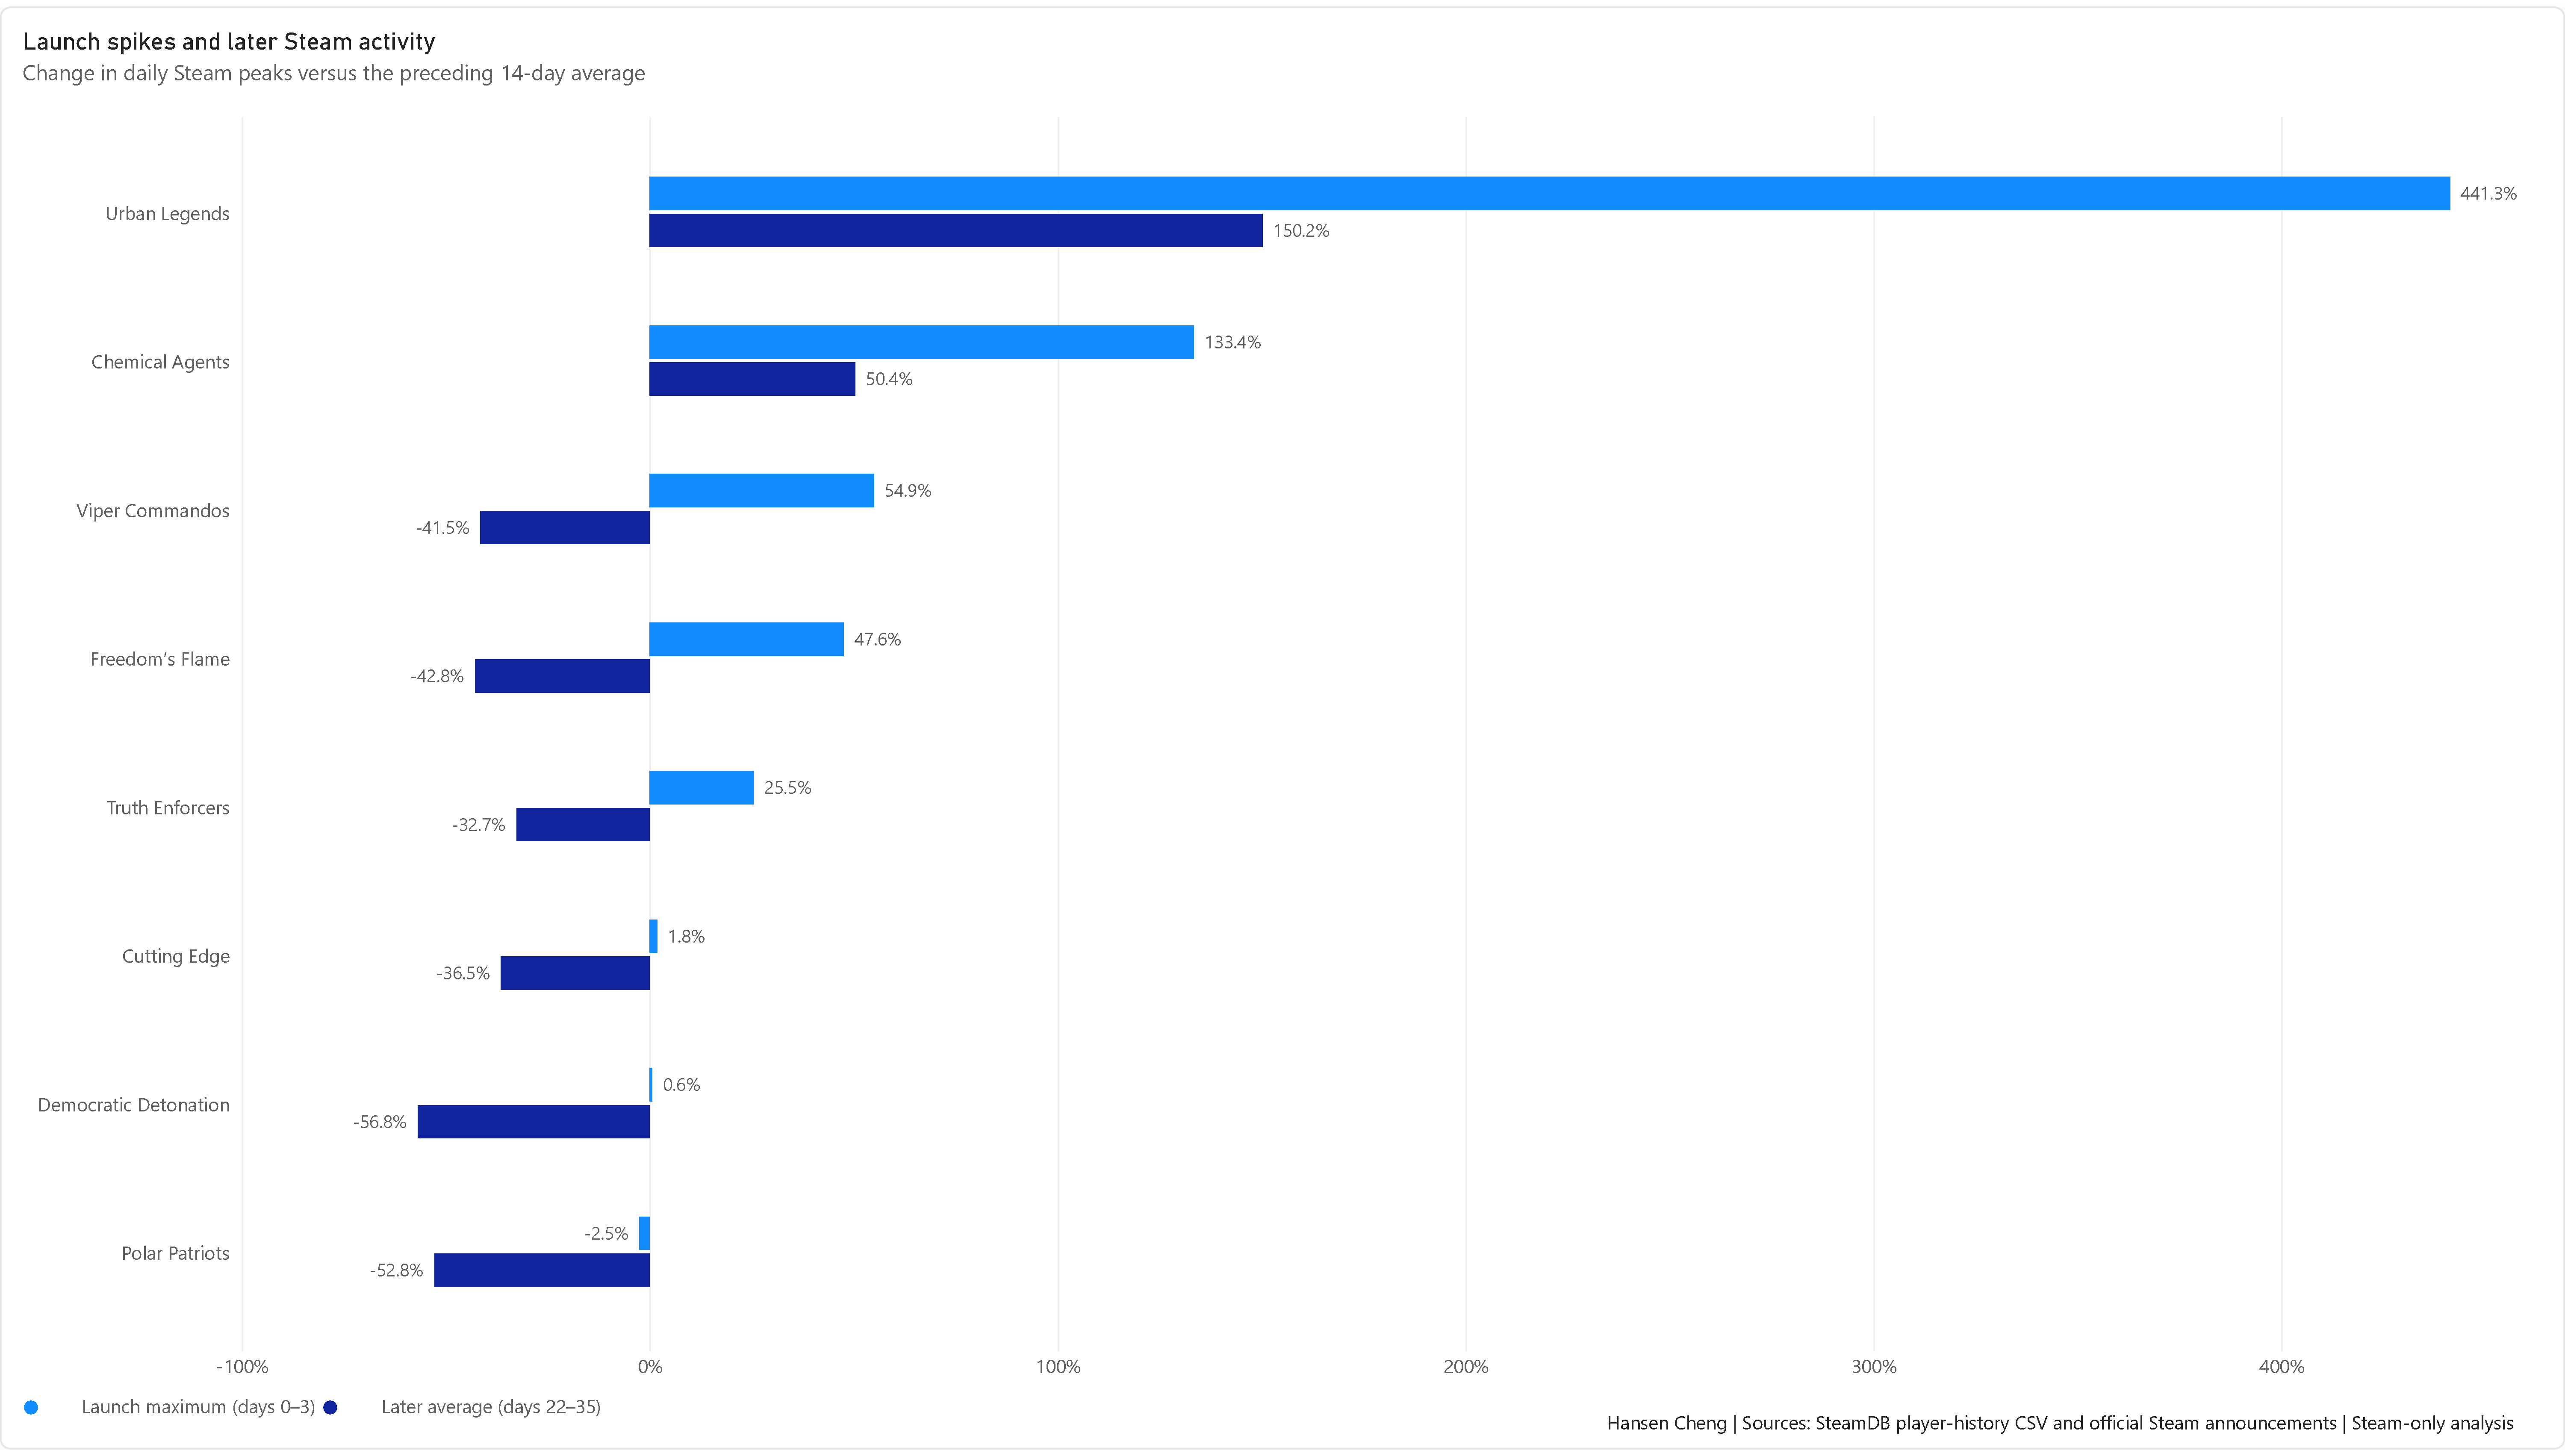
\includepdf[pages=-,pagecommand={\thispagestyle{empty}},width=\paperwidth,height=\paperheight,keepaspectratio]{assets/powerbi-report.pdf}
\end{document}
